\begin{BPMN}{PROC-04}{Elaboración del Plan de Estudios}{}
    \PCitem{Participantes}{}
    \PCitem{Objetivo}{}
    \PCitem{Interrelación con otros procesos}{}
    \PCitem{Proveedores}{}
    \PCitem{Entradas}{}
    \PCitem{Consumidores}{}
    \PCitem{Salidas}{}
    \PCitem{Precondiciones}{}
    \PCitem{Postcondiciones}{}
    \PCitem{Frecuencia}{}
    \PCitem{Tipo}{}
    \PCitem{Áreas de oportunidad}{}
\end{BPMN}
En la figura \hyperref[]{}
\begin{figure}[htbp]
	\begin{center}
	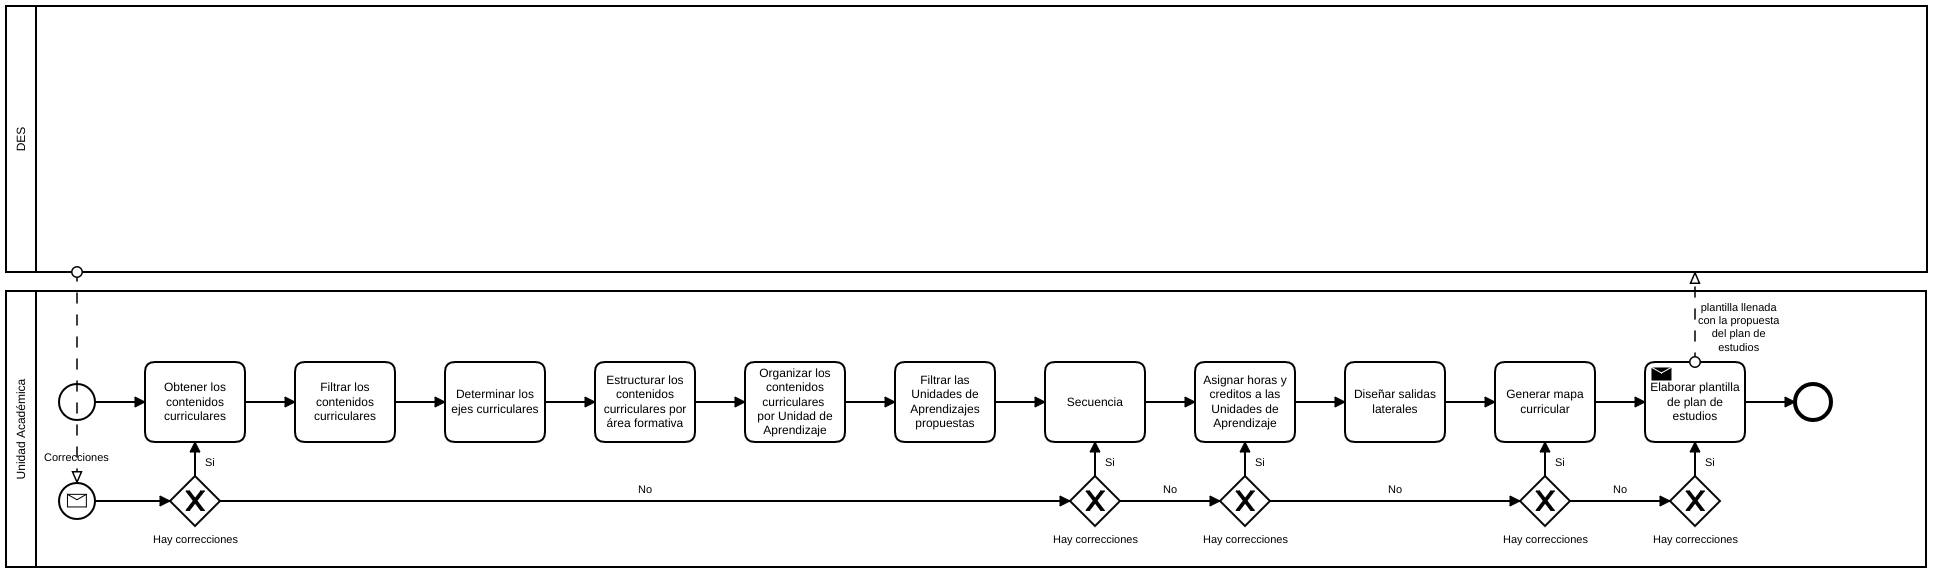
\includegraphics[width=.95\textwidth]{C1-DP/SP4/Image/PlanDeEstudiosBPMN}
		\caption{BPMN-04 Subproceso para la  Elaboración del Plan de Estudios}
		\label{fig:BPMN-04}
	\end{center}
\end{figure}